\newpage
\section{Linear Regression (45 points)}

\subsection{Implement linear regression}
First, we must derive \textbf{w} using QR-decomposition. Starting with:

\begin{align*}
  \mbf{w} &= (\mbf X\T \mbf X)^{-1} \mbf X\T \mbf y\\
\end{align*}

Let $\mbf{QR} = \mbf X$ be the QR-decomposition of $\mbf X$. Then we have:

\begin{align*}
  \mbf{w} &= ((\mbf{QR})\T  \mbf{QR})^{-1} (\mbf{QR})\T \mbf y\\
\end{align*}

Using $(\mbf{QR})\T = \mbf R\T \mbf Q\T$:

\begin{align*}
  \mbf{w} &= (\mbf R\T\mbf Q\T \mbf{QR})^{-1} \mbf R\T\mbf Q\T \mbf y \\
\end{align*}

Since $\mbf Q$ is orthogonal we have $\mbf Q\T \mbf Q = \mbf I$ and thus:

\begin{align*}
  \mbf{w} &= (\mbf R\T\mbf R)^{-1} \mbf R\T\mbf Q\T \mbf y \\
          &= (\mbf R\T\mbf R)^{-1} \mbf R\T\mbf Q\T \mbf y \\
  \mbf R\T\mbf R\mbf{w} &=  \mbf R\T\mbf Q\T \mbf y \\
  \mbf R\mbf{w} &= \mbf Q\T \mbf y \\
\end{align*}

At this point we can either multiply with $\mbf R^{-1}$ on either side of above
equation \textit{or} solve the system of equations $\mbf A \mbf x = \mbf b$,
where $\mbf A = \mbf R$, $\mbf x = \mbf w$, and $\mbf b = \mbf Q\T \mbf y$. Note
that both methods require that $\mbf R$ is non-singular.

Since we want to avoid inverting we choose the latter. In the code this can be
done using \ms{np.linalg.solve}, but since I know \ms R to be a triangular
matrix, I can speed it up using \ms{scipy.linalg.solve_triangular}. My solution
is thus:

\begin{minted}[frame=none]{python}
def fit_qr(X, y):
    X = np.hstack((X, np.ones((X.shape[0], 1)))) # augment X with col of 1's.

    Q, R = np.linalg.qr(X)
    # _w = np.linalg.solve(R, Q.T.dot(y))
    _w = scipy.linalg.solve_triangular(R, Q.T.dot(y))

    return _w[:-1], _w[-1]
\end{minted}

See attached \ms{my_linreg.py} for the full implementation.

\subsection{Building a model}
I build my model(s) in the attached \ms{task_3.py}. The model it pretty
straightforward, since it simply involves transforming the label space with
\ms{np.log()} before running linear regression, and transforming the output
labels with \ms{np.exp()} afterwards, so I will omit the code here.

In any case, the two output parameters I find, as well as the MSE of the model
are:

\begin{align*}
  (a, b) &= (0.259, 0.031),\\
  \text{MSE} &= 34.836.
\end{align*}

Please see \ms{task_3.py} for the actual computations.


\newpage
\subsection{Plot data and model output}
Below figure \ref{fig:3-3} shows the target and model output. Please see
\ms{task_3.py} for model and plotting code.

\begin{figure}[H]
  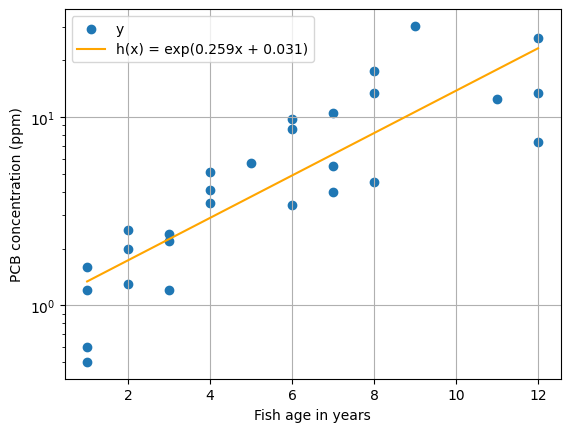
\includegraphics[width=0.9\textwidth]{figures/fig3_3.png}
\caption{Linear model -- $MSE = 34.836$, $R^2 = 0.357$.}
\label{fig:3-3}
\end{figure}

\subsection{Coefficient of determination}

\paragraph{What if $R^2 = 1$?}~\smallskip

If $R^2 = 1$, then the dividend of the quotient must be zero. This is only
possible if $y_i = h(x_i)$ for all $i$, ie. that the model makes a correct
estimation for every $x_i$.

\paragraph{What if $R^2 = 0$?}~\smallskip

If, however, $R^2 = 0$, then the dividend and divisor must be equal, meaning that
on average $h(x_i)$ simply predicts $\bar y$.

\newpage
\paragraph{Can $R^2$ be negative?}~\smallskip

Yes. This happens when the model predictions are even worse than simply
predicting $\bar y$ for every $x_i$, since then the sum of squared errors for
the model is greater than that of simply always guessing $\bar y$.


\paragraph{Computation and discussion of $R^2$ for linear model}~\smallskip

I compute $R^2$ of my model using the formular (please see attached \ms{task_3.py}):

\begin{minted}[linenos=false, frame=none]{python}
  1 - np.sum((y - y_pred) ** 2) / np.sum((y - y_bar) ** 2)}
\end{minted}

and the result is $R^2 = 0.357$. This tells me that my model is at least better
than simply guessing the sample mean, but it is far from being an efficient
estimator.

\subsection{Non-linear model}

I don't change \ms{my_linreg.py}, but rather simply transform the data
before and after running linear regression. Please see \ms{task_3.py}.

\paragraph{MSE and plot of non-linear model}~\smallskip

I run the new non-linear model and get the following model parameters and MSE:

\begin{align*}
  (a, b) &= (1.199, -1.195)\\
  \text{MSE} &= 28.084.
\end{align*}

Again, see \ms{task_3.py} for the actual computations. Below figure
\ref{fig:3-5} shows the target and model output.

\begin{figure}[H]
\centering
  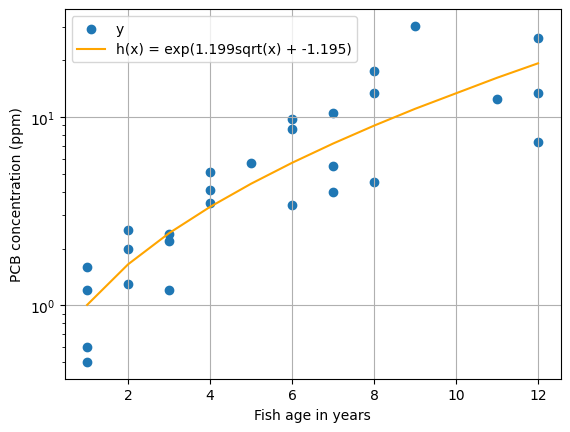
\includegraphics[width=0.9\textwidth]{figures/fig3_5.png}
\caption{Non-linear model -- $MSE = 28.084$, $R^2 = 0.482$}
\label{fig:3-5}
\end{figure}

\paragraph{$R^2$ for the non-linear model}~\smallskip

I compute $R^2$ for my non-linear model to be $R^2 = 0.482$. This is a good step
up from $0.357$ for the linear model, but it is still not particularly good,
since it means my model is only somewhere in the middle between being as good (on
average) as a model that always guesses the sample mean, and a perfectly estimating
model.

\sectend
